\section{Veranstaltungsangebot}

Die Minimalstandards des Veranstaltungsangebots zielen auf die Forderungen
an die Konzeption der mathematikverwandten Studieng"ange.

In jedem ist eine gewisse
fachliche Breite gegeben, und die M"oglichkeit zur Spezialisierung
wird angeboten. Die Entwicklung einer soliden Basis erm"oglicht dem Studenten
die Auswahl der Spezialisierung. Dies bedingt zumindest eine
Auswahl innerhalb der Hochschule oder einen entsprechenden Service der
Vermittlung an entsprechende, hochschulfremde Angebote innerhalb dieses
Schwerpunktes an vergleichbaren Hochschulen.

\begin{kcmt62}
Ist tot.

\subsection{Modelle}

Der Bewertung der "`fachlichen Tiefe"' und "`fachlichen Breite"' innerhalb der "`Minimalstandards"'
liegen zwei Modelle zu Grunde, welche beide auf der KoMa 61 in Regensburg im Konsens entwickelt
wurden. Das erste Modell beinhaltet die verschiedenen Phasen eines
Hochschulstudiums, und erm"oglicht es so, Forderungen an verschiedene Phasen zu
definieren. Das zweite Modell stellt innerhalb eines Fachgebiets ein Modell der
"`Verwandtschaft"' von Themen dar, mit deren Hilfe die Abfolge von Vorlesungen 
und die Konzeption von Studien- und Pr"ufungsordnungen bewertet werden kann.
\end{kcmt62}

\subsection{Phasen des Studiums}

Dem folgenden Modell liegt die Entwicklung des Studenten an der Hochschule zu Grunde. Es beginnt
jedoch schon vor der Immatrikulation.

Die "`nullte"' Phase ist hierbei die Betreuung des Sch"ulers, dessen Information und
ad"aquate Vorbereitung auf ein Hochschulstudium. Darauf folgt die Orientierungsphase
an der Hochschule, die in etwa die ersten beiden Semester beinhaltet. In der
n"achsten Phase erfolgt die Vertiefung der erworbenen Grundf"ahigkeiten.
Abgeschlossen wird das Studium in der Spezialisierungsphase. Die Betreuung
der Studenten endet aber auch hier nicht, die Alumniarbeit sowie Integration und
die weitere Entwicklung der Absolventen an der Hochschule werden auch gef"ordert.

\begin{kcmt}\begin{komacmt}
Die Vorbereitung des Sch"uelers bezieht sich nicht auf den Inhalt des Studiums, sondern die
Informationen was im Studium verlangt wird, zum Beispiel durch Sch"ulerinfotage. Insbesondere ist hier kein Vorkurs gemeint!
\end{komacmt}\end{kcmt}


\begin{center}
	\framebox{\resizebox{.9\textwidth}{!}{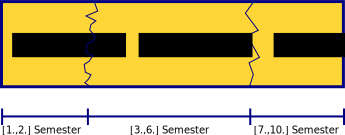
\includegraphics{phasen}}}
\end{center}

\begin{kcmt6XX}

Neue version!

Die Anforderung an die Gestaltung des Angebots eines Studiengangs schlie"st
grunds"atzlich zwei Forderungen ein: gen"ugend "`fachliche Breite"' anzubieten
um eine gute Basis zu schaffen, sowie die M"oglichkeiten eine gewisse
"`fachliche Tiefe"' zu erreichen -- sowohl vor als auch speziell in der Vertiefungsphase
des Studiums.

Hier konkrete Forderungen zu stellen ist uns nicht im Konsens m"oglich, und dies
zeigt auch schon die Freiheit, die den Hochschulen in der Gestaltung ihrer Studieng"ange
nat"urlich vorbehalten bleiben soll. Andererseits k"onnen unsere Forderungen besser
durch folgendes Modell dargestellt werden.

\paragraph{Modell} Dem Modell liegt folgender Gedanke zu Grunde: "`Gehen wir einmal davon
aus, dass F"acher bzw. Themengebiete eine Metrik h"atten."' Als Beispiel sei hier eine
"`Messung"' der Distanz zwischen bspw. "`reiner"' und "`angewandter"' Mathematik, oder
eine zwischen "`Lineare Algebra I"', "`Lineare Algebra II"' und "`Analysis"' genannt. Durch diese Metrik
lassen sich Umgebungen finden, die verschiedene Themengebiete der Mathematik umfassen
und sich thematisch "`eng"' gruppieren. Weiterhin entstehen durch behandelte, "`entfernte"'
Themengebiete neue "`Dimensionen"'. Folgendes Beispiel soll dies verdeutlichen:

\begin{center}
\framebox{\resizebox{.75\textwidth}{!}{\includegraphics{dimensionen}}}
\end{center}

Dieses Beispiel zeigt eine m"ogliche Grundausbildung, welche f"ur gen"ugend "`fachliche
Breite"' sorgt, sowie mehrere verschiedene potentielle Zuk"unfte f"ur den Studierenden
-- an dieser Hochschule oder anderswo -- mit Schwerpunkten in verschiedenen Bereichen.

Der Nullpunkt stellt hier das erworbene Wissen innerhalb des Studiengebietes dar.
Mit der Zeit, w"ahrend die Studierenden durch die verschiedenen Phasen ihres Studiums
fortschreiten, entwickeln sie sich auf den verschiedenen Skalen (Dimensionen)
vorw"arts. Hier kommt auch wieder die Konzeption der Studieng"ange ins Spiel, speziell
inwiefern verschiedene Skalen angeboten werden, wieviele verpflichtend und optional
sind, wie weit sich Studierende weiterentwickeln k"onnen etc.

Mit diesen beiden Modellen vor Augen k"onnen die Minimalstandards formuliert werden.
Diese schlie"st auch eine gewisse Mobilit"at, Autonomie und Engagement
der Studierenden mit ein; dieses wird jedoch von der Hochschule sowohl erm"oglicht
als auch gef"ordert.

Es ist nicht Aufgabe der Minimalstandards einen F"acherkatalog bzw. curriculare
Vorschl"age darzubieten. Dies geschieht stattdessen im Rahmen der Hochschulen und
ihrer Koordination untereinander.

\begin{kcmt62}
\begin{komacmt62}
\begin{eqnarray*}
	dim(V) \geq & n \\
	n > & 1 \\
	Geg. \epsilon > & 0:\\
	\forall  v \in V & \exists u \in V_\epsilon(v) \backslash \{v\}
\end{eqnarray*}

Diese Formeln hier sind aus dem Dokument gewandert weil sie f"ur zuviel
Verwirrung sorgen. Zwar l"a"st sich die Anforderung an den Studiengang
so zweifelsfrei formulieren, andererseits aber ist diese Formulierung
nicht leicht verst"andlich.
\end{komacmt62}
\end{kcmt62}

\begin{kcmt62}
\begin{komacmt62}
Folgendes wird durch die Arbeit von Karin \& Co. ersetzt:

Das hei"st es werden mindestens zwei Themengebiete der Mathematik an der Hochschule
abgedeckt. Weiterhin existiert eine maximale Spanne zwischen den verwandten
Gebieten, was bedeutet das eine kontinuierliche Weiterentwicklung der F"ahigkeiten
und Kenntnisse der Studierenden im ausgew"ahlten Gebiet stattfindet -- die Vorlesungen
entwickeln sich sozusagen "`stetig"' und bauen aufeinander -- im Sinne der Skala dieser
"`Dimension"' der Mathematik -- auf.
\end{komacmt62}
\end{kcmt62}

\end{kcmt6XX}

\newpage
\subsection{Diversit"at und Spezialisierung}

Die Anforderung an die Gestaltung des Angebots eines Studiengangs schlie"st grunds"atzlich zwei Forderungen ein: 
\begin{enumerate}
	\item Gen"ugend "`fachliche Breite"' anzubieten, um eine gute Basis zu schaffen.
	\item Die M"oglichkeiten eine gewisse "`fachliche Tiefe"' zu erreichen -- sowohl vor als auch speziell in der Vertiefungsphase des Studiums.
\end{enumerate}

Um die abstrakten Begriffe "`fachliche Tiefe"' und "`fachliche
Breite"' fassen zu k"onnen, verwenden wir ein Modell zur Einordnung
der verschiedenen Lehrveranstaltungen bzw. zur Beschreibung ihrer
Beziehung untereinander.  Eine Veranstaltung l"asst sich mindestens
einem Bereich (Richtung) der Mathematik zuordnen. Diese Richtungen
spannen als Achsen den Raum der m"oglichen Veranstaltungen auf.
Hierbei entspricht der Nullpunkt dem Wissensstand eines Studienanf"angers.
Die Entfernung einer Veranstaltung vom Nullpunkt ist ein Ma"s f"ur
die fachliche Tiefe, die sie einem Studenten verleiht.

\begin{center}
\textbf{Ein Beispiel}\\
\framebox{\resizebox{.75\textwidth}{!}{\includegraphics{dimensionen}}}
\end{center}

\newpage
Im Folgenden werden die Minimalstandards der Diversit"at und Spezialisierung formuliert:
\begin{enumerate}
\item Eine Hochschule bietet mindestens zwei unterschiedliche fachliche Richtungen innerhalb der Mathematik an.

\item Wenn eine (weiterf"uhrende) Veranstaltung Wissen voraussetzt,
welches "uber den Wissensstand eines Studienanf"angers hinausgeht,
wird zeitnah eine Veranstaltung angeboten, die dieses Wissen zuvor vermittelt.

\item In mindestens zwei der angebotenen Richtungen gibt es gen"ugend
weiterf"uhrende Veranstaltungen, so dass eine kontinuierliche
Weiterentwicklung der F"ahigkeiten und Kenntnisse des Studenten
stattfindet.

Hierzu geh"ort: Er lernt in mindestens zwei Richtungen seiner Wahl
Zusammenh"ange seines Faches zu "uberblicken und selbstst"andig
mathematische Methoden auszuw"ahlen und sachgerecht anzuwenden.
Des Weiteren lernt er, sich selbstst"andig in verwandte neue Themen
einzulesen und diese nachzuvollziehen.
\end{enumerate}

Diese Forderungen gehen auch von einer gewissen Mobilit"at, Autonomie
und einem Engagement des Studenten aus; dieses wird von
der Hochschule sowohl erm"oglicht als auch gef"ordert.

Es ist nicht Aufgabe der Minimalstandards, einen F"acherkatalog bzw.
curriculare Vorschl"age darzubieten. Dies geschieht stattdessen im
Rahmen der Hochschulen und ihrer Koordination untereinander.




\subsection{Erste Studienphase}

Der
Student kommt an die Hochschule und durchl"auft zun"achst eine Orientierungsphase.
W"ahrend dieser gew"ohnt er sich an das Lern- und Arbeitsniveau der Hochschule und
findet sich fachlich, sowohl was die Affinit"at zu etwaigen pers"onlichen Schwerpunkten
als auch was das gesamte mathematische Angebot anbelangt, in der Hochschule ein.

In der ersten Phase des Studiums wird der Student an das Fachgebiet herangef"uhrt.
Durch Schaffen einer soliden Basis wird sowohl die Vertiefung ausgew"ahlter Themen
erm"oglicht als auch die Autonomie gest"arkt, indem der sp"ateren Auswahl der
Spezialthemen ein solides Fundament unterstellt wird.

Hierbei wird auch auf Schwankungen bei den Vorkenntnissen der Studenten
eingegangen, d.h. nach Abschluss der ersten Studienphase sind eventuell 
vorhandene M"angel erkannt und ausgeglichen.

In der ersten Phase des Studiums wird noch keine Vertiefung erwartet; hier werden
die Richtungen geschaffen, und erste Schritte innerhalb dieser gemacht.
Der Student wird hierbei mit den an der Hochschule behandelten Themengebieten
vertraut gemacht (siehe Vorlesungen, Seite \pageref{vorlesung:anforderungen}).

Nach dieser Phase kann ein Student mit m"oglichst geringem Aufwand die Hochschule
bzw. den Studiengang wechseln.


\subsection{Zweite Studienphase}

Der Student hat inzwischen ein fachliches Basisniveau erreicht und
kann schon erkennen, welche Vertiefungsm"oglichkeiten an der eigenen Hochschule angeboten
werden und wie auf diese hingef"uhrt wird.
Im Rahmen dieser Studienphase wird er zur Auswahl der Schwerpunkte bef"ahigt. 

In der zweiten Studienphase finden in ausgew"ahlten Richtungen Vertiefungen statt,
eine weitere Spezialisierung des Studenten wird vorbereitet. Um den Studenten Vertiefungen in verschiedene Richtungen zu erm"oglichen, unterst"utzt die Hochschule
in dieser Phase auch Hochschulwechsel.
Bei diesen werden bereits erbrachte gleichwertige Leistungen anerkannt.
Bei abweichenden Studieng"angen muss
aber auch der Student Aufwand einplanen um sich dem Curriculum der neuen
Hochschule anzupassen.

Ein Studienwechsel wird durch die Hochschule zumindest soweit unterst"utzt, dass auf Anfrage eines Studenten Informationen "uber die gew"unschte Vertiefung an anderen Hochschulen bereitgestellt werden. Die Hochschule, an die gewechselt wird, stellt auf Anfrage klar, welche Leistungen anerkannt werden und welche Leistungen nachzuholen sind.

In dieser Phase wird sowohl die fachliche Breite als auch die fachliche Tiefe gef"ordert.

\subsection{Dritte Studienphase}

Ein Student der dritten Phase kann schon einen ersten Hochschulabschluss besitzen
und ist in der Lage, selbstst"andig wissenschaftlich zu arbeiten sowie autonom seine Spezialisierung
auszuw"ahlen und voranzutreiben. Nach der dritten Phase besitzt er die F"ahigkeit,
mathematische Methoden und wissenschaftliche Erkenntnisse selbstst"andig anzuwenden.

Hierbei wird dem Studenten erm"oglicht, sich in den von ihm gew"ahlten Richtungen
weiter zu vertiefen.

Ist keine dritte Phase vorhanden, kann mit Abschluss der zweiten Phase ohne Verl"angerung der Gesamtstudienzeit die dritte Phase an einer anderen Hochschule absolviert werden. Informationen "uber geeignete Hochschulen sind dem Studenten rechtzeitig bekannt zu geben.


\subsection{Kontinuit"at}

Ein Studium ist, gleich welche der angebotenen Richtungen der Student w"ahlt, 
in der Regelstudienzeit absolvierbar.

\begin{kcmt}\begin{komacmt}
Wenn der Student eine bestimmt Vertiefungsrichtung, die an der Hochschule
angeboten wird, studieren m"ochte, so kann er dies unabh"angig von seinem Studienbeginn 
tun. z.B. BA-Arbeit, auf der Zyklus nicht eingestellt war. Vorlesungszyklen, die nicht 
regelm"a"sig angeboten werden. Die Wdh- Rate der Zyklen darf die Gesamtstudienzeit nicht beeinflussen
\end{komacmt}\end{kcmt}

Aufeinander aufbauende Studieng"ange sind in Regelstudienzeit absolvierbar,
insbesondere wirkt sich der "Ubergang von einem Studiengang in einen darauf aufbauenden Studiengang nicht notwendig verl"angernd 
auf die Gesamtstudienzeit aus.

\begin{kcmt}\begin{komacmt}
Damit sollen eventuelle L"ucken vermieden werden, die sich aus der strukturellen 
Eigenschaften des BA-Stud. ergeben. Kern, BA + MA = 10 Semester regel. Problem: 
BA-Arbeit nicht in Zyklen eingeplant.
\end{komacmt}\end{kcmt}

Die Umsetzung der Studienordnung, insbesondere das Vorlesungsangebot und die 
Pr"ufungsordnungen, ist so flexibel gestaltet, dass Abweichungen vom planm"a"sigen 
Studienverlauf das Gesamtstudium nicht unverh"altnism"a"sig verl"angern. 
Speziell zieht ein Ausfall von einem Semester h"ochstens eine Studienzeitverl"angerung 
von zwei Semestern nach sich.

\begin{kcmt}\begin{komacmt}
Ausfallgr"unde: Krankheit, Unfall, Auslandssemester, private Probleme, sonst. Zielt wieder auf Zyklen ab.


Allgemein sehen wir es als schwierig an, wenn auf die bisherige Zyklen-Anordnung eine 
BA-MA Struktur ohne Anpassung gest"ulpt wird (Stichwort Aussetzen von einem Semster 
wg. BA-Arbeit und weiterlaufen des Zykluses) Vorlesungszyklen o."a m"ussen an die 
strukturellen Gegebenheiten angepasst werden. 
\end{komacmt}\end{kcmt}

\subsection{Teilzeitstudium / Studieren mit Kind}

Ein Beispielstudiengangsverlauf ist angegeben, bei dem die maximale Arbeitsbelastung 
pro Semester ein gewisses H"ochstma"s (Richtlinie: Alleinerziehendes Elternteil) nicht 
"ubersteigt. Dabei sind keine besonderen Vorkenntnisse gefordert, insbesondere ist auch
die Studiengeb"uhrensituation beachtet. Unter Ber"ucksichtigung dieser Rahmenbedingungen
entsteht dem Studenten bei Einhaltung dieses Beispielstudienverlaufs kein finanzieller
Nachteil.

\begin{kcmt}\begin{komacmt}
Ein Teilzeitstudium muss in angemessener Zeit schaffbar sein. Das Verh"altnis 
Semesterbelastung / Studienl"ange soll ungef"ahr gleich bleiben. 
Hier m"ussen noch konkrete Zahlen gefunden werden. 
\end{komacmt}\end{kcmt}

\subsection{Pr"ufungen}

Bei benoteten Modulen wird zu Beginn der einzelnen Veranstaltung(en) die Bewertungsmethode 
transparent gemacht. Insbesondere gilt f"ur Module, die mehrere Veranstaltungen 
oder Submodule beinhalten, dass dies mit Beginn der ersten Veranstaltung vorgestellt wird.
Mit Einverst"andnis aller Teilnehmer kann das System auch w"ahrend des Moduls ge"andert werden. 

Wenn das Nichtbestehen einer Pr"ufung einen Studienausschluss zur Folge hat, so 
wird dem Studenten die M"oglichkeit gegeben, die Pr"ufung mindestens zweimal
zu wiederholen. Dem Studenten wird die M"oglichkeit gegeben, die Pr"ufung 
so zu wiederholen, dass es zu keiner Verz"ogerung in seinem Studienverlauf kommt. 
Andererseits wird dem Studenten die M"oglichkeit gegeben, die Pr"ufung entweder
z"ugig zu wiederholen oder vor einer erneuten Pr"ufung pr"ufungsrelevante Veranstaltungen
erneut zu besuchen.

\begin{kcmt}\begin{komacmt}
Diese beiden Versuchen schlie"sen sich gegenseitig nicht aus.
\end{komacmt}\end{kcmt}

Werden Pr"ufungstermine vorgegeben, so sind diese mindestens einen Monat im voraus
anzuk"undigen.
\begin{kcmt}\begin{komacmt}
	Dies zielt auf zentrale Klausuren und nicht 
	auf individuelle Absprachen ab

	Wir beschr"anken uns erstmal nur auf Pr"ufungen, die im negativen Fall 
	einen Ausschluss vom Studium zur Folge haben.  Unsere Forderungen implizieren 
	insbesondere, das bei Modulen, deren Bestehen f"ur weitere Module Vorausssetzung 
	ist, ggf. mehr Wiederholungstermine angeboten werden m"usssen. 
\end{komacmt}\end{kcmt}

\subsubsection{Schriftliche Arbeiten}

Schriftliche Arbeiten werden von einem Studenten eigenst"andig angefertigt.
Bei einem umfangreichen Thema kann dieses auch entsprechend von mehr Studenten gemeinsam bearbeitet werden.
Jeder Student wird von einer fachlich kompetenten Person betreut.
Der Betreuer ist zu mindestens einem monatlichen pers"onlichen Gespr"ach bereit.
Zus"atzlich ist er f"ur kurze Nachfragen jederzeit erreichbar und antwortet auf diese innerhalb einer Woche.

Das zu behandelnde Thema wird zu Beginn der Arbeit festgelegt.
Die vom Studenten ge"au"serten Interessen werden bei der Vergabe des Themas ber"ucksichtigt.
Auf Wunsch des Studenten erfolgt die Vergabe des Themas so rechtzeitig, dass das Studium nicht unn"otig verl"angert wird.
Der Umfang des Themas wird so gew"ahlt, dass die Arbeit im daf"ur vorgesehenen Zeitrahmen fertiggestellt werden kann.


\subsection{Kontinuit"at der Studienordnung}

Jedem Studenten, der in einer Studienordnung beginnt, ist es m"oglich, in dieser sein Studium auch abzuschlie"sen.

Dies gilt insbesondere, wenn die Studienordnung ausl"auft.
In diesem Fall hat er f"ur das erfolgreiche Abschlie"sen des Studiums ab dem Zeitpunkt, zu dem keine Neueinschreibung gem"a"s dieser Studienordnung mehr m"oglich ist, Regelstudienzeit plus ein Jahr Zeit.
Sofern eine neuere Studienordnung existiert, ist es dem Studenten jederzeit m"oglich, auf diese wechseln.
Die bereits erbrachten Leistungen werden gem"a"s klar formulierten "Ubergangsregelungen (z.B. einer "Aquivalenzliste) anerkannt.

\begin{kcmt}\begin{komacmt}
	Gesetzliche Vorschrift nochmal erw"ahnen. Wenn ich in einer Studienordnung 
	beginne, musss ich mit dieser auch beenden k"onnen. Insbesondere, wenn es ein wenig l"anger dauert.
\end{komacmt}\end{kcmt}

\begin{stilltodo}
\subsection{Autonomie}

{\Large{Still To Do.}}
\end{stilltodo}

\subsection{Freiheit des Lernens}

Der Student ist selbstst"andig und "ubernimmt Eigenverantwortung. Die Hochschule
unterst"utzt ihn in der Freiheit, seinen Studienverlauf selbst zu gestalten.
Das umfasst sowohl die Anordnung der Veranstaltungen als auch die Wahl der Methodik
und Sozialform des Lernens, wie z.B. Autodidaktik.

Grunds"atzlich widerspricht Anwesenheitspflicht bei Veranstaltungen dem Gedanken
der Freiheit des Lernens, einzige Ausnahme k"onnen Seminare darstellen. Wenn Zulassungsvoraussetzungen
zur Pr"ufung einer Veranstaltung existieren, dann sind diese nur innerhalb dieser
Veranstaltung zu erbringen.

Die Wahl des Zeitpunkts des Studienabschlusses ist dem Studenten "uberlassen.

\begin{kcmt}\begin{komacmt}
	Gegenst"uck zur Verschulung. Selbstverantwortung der Studierenden. Wahlm"oglichkeiten alleine reichen nicht aus.
\end{komacmt}\end{kcmt}

\subsection{Orientierung an den Interessen der Studierenden}
Dem Studenten wird die M"oglichkeit gegeben, das Veranstaltungsangebot mitzugestalten. 
Dies bedeutet, dass in allen Gremien, welche Studien- und Pr"ufungsordnungen oder die 
Vorlesungsverzeichnisse beschlie"sen, Studenten mit Stimmrecht vertreten sind. Diese sind
durch die Fachschaft zu w"ahlen.

\begin{kcmt}\begin{komacmt}
Er muss die M"oglichkeit bieten, Fehlendes aus einem BA Studium nachzuholen -> Kontinuit"at
\end{komacmt}\end{kcmt}

\begin{kcmt}\begin{komacmt}
\paragraph{Noch fehlend}
\begin{itemize}
 \item fachliche Breite definieren
 \item Autodidaktisches Studium
 \item Beispielstudienverl"ufe
\end{itemize}
\end{komacmt}\end{kcmt}
